\documentclass{standalone}
\usepackage{tikz}
\usetikzlibrary{patterns, positioning}


\begin{document}
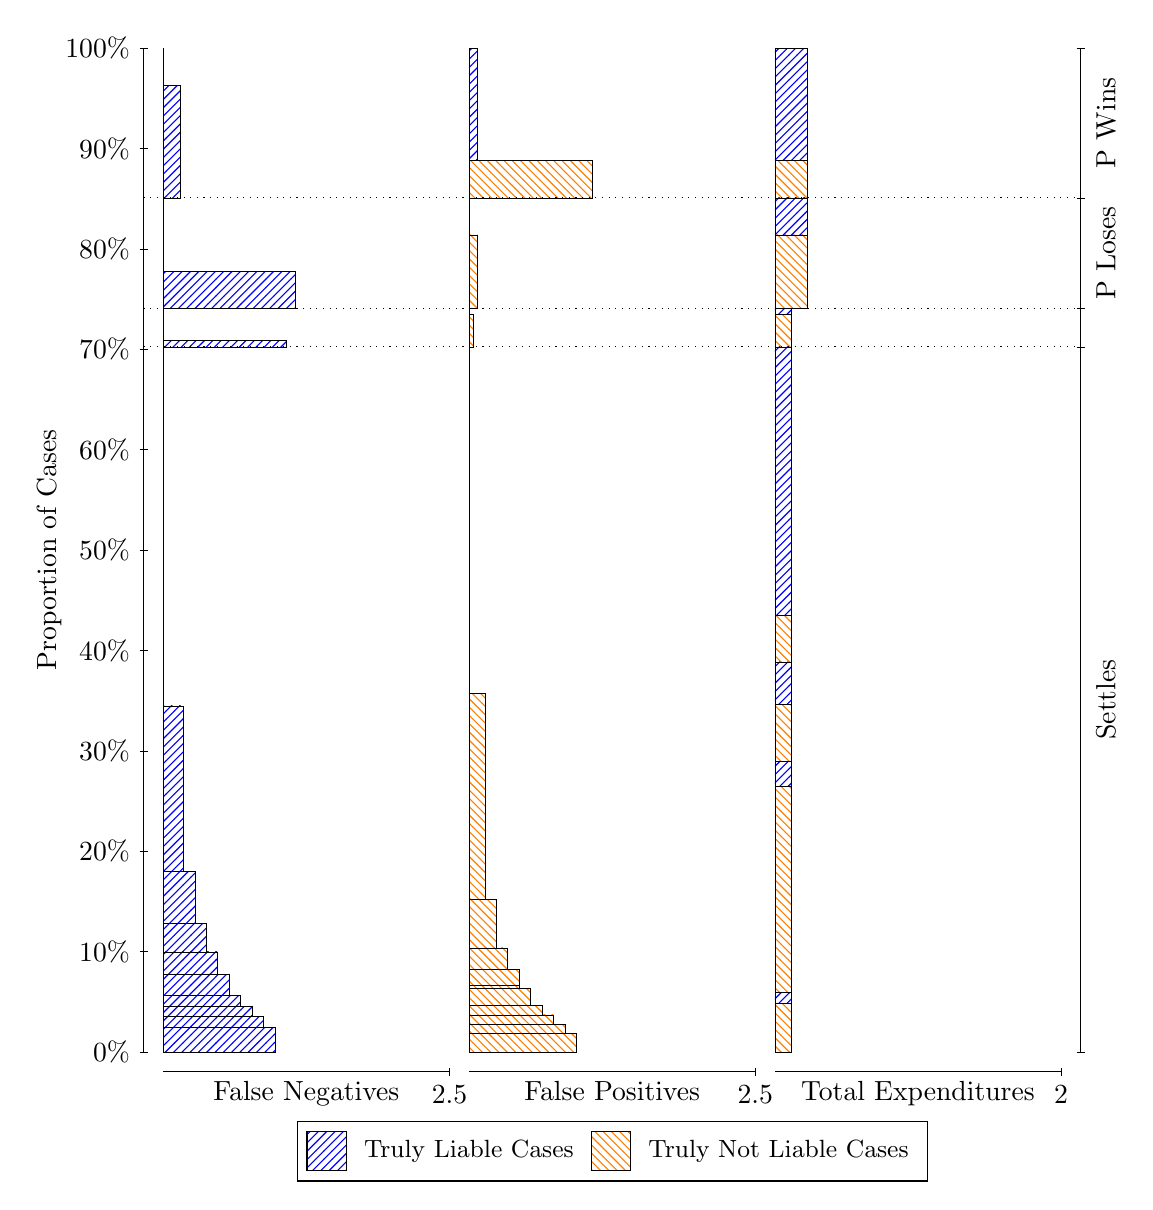
\begin{tikzpicture}
\draw[black, very thin] (1.5,1.75) -- (1.5,14.5);
\node[rotate=90, text=black, anchor=center] at (0.3, 8.125) {Proportion of Cases};
\draw[black, very thin] (1.45,1.75) -- (1.55,1.75);
\node[text=black, anchor=east] at (1.45, 1.75) {0\%};
\draw[black, very thin] (1.45,3.025) -- (1.55,3.025);
\node[text=black, anchor=east] at (1.45, 3.025) {10\%};
\draw[black, very thin] (1.45,4.3) -- (1.55,4.3);
\node[text=black, anchor=east] at (1.45, 4.3) {20\%};
\draw[black, very thin] (1.45,5.575) -- (1.55,5.575);
\node[text=black, anchor=east] at (1.45, 5.575) {30\%};
\draw[black, very thin] (1.45,6.85) -- (1.55,6.85);
\node[text=black, anchor=east] at (1.45, 6.85) {40\%};
\draw[black, very thin] (1.45,8.125) -- (1.55,8.125);
\node[text=black, anchor=east] at (1.45, 8.125) {50\%};
\draw[black, very thin] (1.45,9.4) -- (1.55,9.4);
\node[text=black, anchor=east] at (1.45, 9.4) {60\%};
\draw[black, very thin] (1.45,10.675) -- (1.55,10.675);
\node[text=black, anchor=east] at (1.45, 10.675) {70\%};
\draw[black, very thin] (1.45,11.95) -- (1.55,11.95);
\node[text=black, anchor=east] at (1.45, 11.95) {80\%};
\draw[black, very thin] (1.45,13.225) -- (1.55,13.225);
\node[text=black, anchor=east] at (1.45, 13.225) {90\%};
\draw[black, very thin] (1.45,14.5) -- (1.55,14.5);
\node[text=black, anchor=east] at (1.45, 14.5) {100\%};

\draw[black, very thin] (13.4,1.75) -- (13.4,14.5);
\draw[black, very thin] (13.35,1.75) -- (13.45,1.75);
\node[anchor=west] at (13.35, 1.75) {};
\draw[black, very thin] (13.35,10.704) -- (13.45,10.704);
\node[anchor=west] at (13.35, 10.704) {};
\draw[black, very thin] (13.35,11.196) -- (13.45,11.196);
\node[anchor=west] at (13.35, 11.196) {};
\draw[black, very thin] (13.35,12.598) -- (13.45,12.598);
\node[anchor=west] at (13.35, 12.598) {};
\draw[black, very thin] (13.35,14.5) -- (13.45,14.5);
\node[anchor=west] at (13.35, 14.5) {};

\draw[black, very thin, pattern color=blue, pattern=north east lines] (1.75,1.75) rectangle (3.167,2.0613);
\draw[black, very thin, pattern color=blue, pattern=north east lines] (1.75,2.0613) rectangle (3.0217,2.1988);
\draw[black, very thin, pattern color=blue, pattern=north east lines] (1.75,2.1988) rectangle (2.8763,2.3329);
\draw[black, very thin, pattern color=blue, pattern=north east lines] (1.75,2.3329) rectangle (2.731,2.4668);
\draw[black, very thin, pattern color=blue, pattern=north east lines] (1.75,2.4668) rectangle (2.5857,2.7332);
\draw[black, very thin, pattern color=blue, pattern=north east lines] (1.75,2.7332) rectangle (2.4403,3.0214);
\draw[black, very thin, pattern color=blue, pattern=north east lines] (1.75,3.0214) rectangle (2.295,3.3808);
\draw[black, very thin, pattern color=blue, pattern=north east lines] (1.75,3.3808) rectangle (2.1497,4.0438);
\draw[black, very thin, pattern color=blue, pattern=north east lines] (1.75,4.0438) rectangle (2.0043,6.146);
\draw[black, very thin, pattern color=orange, pattern=north west lines] (1.75,6.146) rectangle (1.75,10.704);
\draw[black, very thin, pattern color=blue, pattern=north east lines] (1.75,10.704) rectangle (3.3123,10.784);
\draw[black, very thin, pattern color=orange, pattern=north west lines] (1.75,10.784) rectangle (1.75,11.196);
\draw[black, very thin, pattern color=blue, pattern=north east lines] (1.75,11.196) rectangle (3.4213,11.667);
\draw[black, very thin, pattern color=orange, pattern=north west lines] (1.75,11.667) rectangle (1.75,12.598);
\draw[black, very thin, pattern color=blue, pattern=north east lines] (1.75,12.598) rectangle (1.968,14.027);
\draw[black, very thin, pattern color=orange, pattern=north west lines] (1.75,14.027) rectangle (1.75,14.5);
\draw[black, very thin, pattern color=orange, pattern=north west lines] (5.6333,1.75) rectangle (6.9958,1.9813);
\draw[black, very thin, pattern color=orange, pattern=north west lines] (5.6333,1.9813) rectangle (6.8505,2.0973);
\draw[black, very thin, pattern color=orange, pattern=north west lines] (5.6333,2.0973) rectangle (6.7052,2.2216);
\draw[black, very thin, pattern color=orange, pattern=north west lines] (5.6333,2.2216) rectangle (6.5598,2.338);
\draw[black, very thin, pattern color=orange, pattern=north west lines] (5.6333,2.338) rectangle (6.4145,2.5606);
\draw[black, very thin, pattern color=orange, pattern=north west lines] (5.6333,2.5606) rectangle (6.2692,2.5953);
\draw[black, very thin, pattern color=orange, pattern=north west lines] (5.6333,2.5953) rectangle (6.2692,2.8032);
\draw[black, very thin, pattern color=orange, pattern=north west lines] (5.6333,2.8032) rectangle (6.1238,3.0707);
\draw[black, very thin, pattern color=orange, pattern=north west lines] (5.6333,3.0707) rectangle (5.9785,3.6924);
\draw[black, very thin, pattern color=orange, pattern=north west lines] (5.6333,3.6924) rectangle (5.8332,6.3082);
\draw[black, very thin, pattern color=blue, pattern=north east lines] (5.6333,6.3082) rectangle (5.6333,10.704);
\draw[black, very thin, pattern color=orange, pattern=north west lines] (5.6333,10.704) rectangle (5.6878,11.117);
\draw[black, very thin, pattern color=blue, pattern=north east lines] (5.6333,11.117) rectangle (5.6333,11.196);
\draw[black, very thin, pattern color=orange, pattern=north west lines] (5.6333,11.196) rectangle (5.7423,12.128);
\draw[black, very thin, pattern color=blue, pattern=north east lines] (5.6333,12.128) rectangle (5.6333,12.598);
\draw[black, very thin, pattern color=orange, pattern=north west lines] (5.6333,12.598) rectangle (7.1957,13.071);
\draw[black, very thin, pattern color=blue, pattern=north east lines] (5.6333,13.071) rectangle (5.7423,14.5);
\draw[black, very thin, pattern color=orange, pattern=north west lines] (9.5167,1.75) rectangle (9.721,2.3717);
\draw[black, very thin, pattern color=blue, pattern=north east lines] (9.5167,2.3717) rectangle (9.721,2.5093);
\draw[black, very thin, pattern color=orange, pattern=north west lines] (9.5167,2.5093) rectangle (9.721,5.1251);
\draw[black, very thin, pattern color=blue, pattern=north east lines] (9.5167,5.1251) rectangle (9.721,5.4364);
\draw[black, very thin, pattern color=orange, pattern=north west lines] (9.5167,5.4364) rectangle (9.721,6.169);
\draw[black, very thin, pattern color=blue, pattern=north east lines] (9.5167,6.169) rectangle (9.721,6.7034);
\draw[black, very thin, pattern color=orange, pattern=north west lines] (9.5167,6.7034) rectangle (9.721,7.2914);
\draw[black, very thin, pattern color=blue, pattern=north east lines] (9.5167,7.2914) rectangle (9.721,10.704);
\draw[black, very thin, pattern color=orange, pattern=north west lines] (9.5167,10.704) rectangle (9.721,11.117);
\draw[black, very thin, pattern color=blue, pattern=north east lines] (9.5167,11.117) rectangle (9.721,11.196);
\draw[black, very thin, pattern color=orange, pattern=north west lines] (9.5167,11.196) rectangle (9.9254,12.128);
\draw[black, very thin, pattern color=blue, pattern=north east lines] (9.5167,12.128) rectangle (9.9254,12.598);
\draw[black, very thin, pattern color=orange, pattern=north west lines] (9.5167,12.598) rectangle (9.9254,13.071);
\draw[black, very thin, pattern color=blue, pattern=north east lines] (9.5167,13.071) rectangle (9.9254,14.5);
\draw[black, dotted] (1.5,10.704) -- (13.4,10.704);
\draw[black, dotted] (1.5,11.196) -- (13.4,11.196);
\draw[black, dotted] (1.5,12.598) -- (13.4,12.598);
\draw[black, very thin] (1.75,1.5) -- (5.3833,1.5);
\node[text=black, anchor=north] at (3.5667, 1.5) {False Negatives};
\draw[black, very thin] (5.3833,1.45) -- (5.3833,1.55);
\node[text=black, anchor=north] at (5.3833, 1.45) {2.5};

\draw[black, very thin] (5.6333,1.5) -- (9.2667,1.5);
\node[text=black, anchor=north] at (7.45, 1.5) {False Positives};
\draw[black, very thin] (9.2667,1.45) -- (9.2667,1.55);
\node[text=black, anchor=north] at (9.2667, 1.45) {2.5};

\draw[black, very thin] (9.5167,1.5) -- (13.15,1.5);
\node[text=black, anchor=north] at (11.333, 1.5) {Total Expenditures};
\draw[black, very thin] (13.15,1.45) -- (13.15,1.55);
\node[text=black, anchor=north] at (13.15, 1.45) {2};

\node[text=black, centered, rotate=90] at (13.72, 6.2271) {Settles};

\node[text=black, centered, rotate=90] at (13.72, 11.897) {P Loses};
\node[text=black, centered, rotate=90] at (13.72, 13.549) {P Wins};

\draw (7.449999999999999,1.5) node[draw=none] (baseCoordinate) {};
\begin{scope}[align=center]
        \matrix[scale=0.5, draw=black, below=0.5cm of baseCoordinate, nodes={draw}, column sep=0.1cm]{
            \node[rectangle, draw, minimum width=0.5cm, minimum height=0.5cm, pattern color=blue, pattern=north east lines] {}; &
            \node[draw=none, font=\small, text=black] (B) {Truly Liable Cases}; &
            \node[rectangle, draw, minimum width=0.5cm, minimum height=0.5cm, pattern color=orange, pattern=north west lines] {}; &
            \node[draw=none, font=\small, text=black] (B) {Truly Not Liable Cases}; \\
            };
\end{scope}

\end{tikzpicture}
\end{document}